\chapter{Plataforma de desarrollo}
\label{cap:capitulo3}

\vspace{0.25cm}

\section{Introducción}
\label{sec:segundaseccion}

En este capítulo se presenta una visión global del sistema desarrollado en este TFG, ofreciendo una descripción del CDPR diseñado y de toda la arquitectura que hace posible su funcionamiento, la cual ha permitido validar el modelo cinemático, así como los algoritmos para planificar trayectorias utilizados y su integración en ROS 2. Y aunque gran parte del sistema hardware se encuentre en una fase preliminar, todo su diseño se está teniendo en cuenta desde el principio.

\section{Funcionamiento de un CDPR bidimensional}
\label{sec:segundaseccion}

El funcionamiento principal de un CDPR bidimensional consiste en el desplazamiento de un efector final, dentro de una región del mismo tipo que el robot, todo ello mediante el accionamiento de dos cables, donde cada uno de ellos conecta el efector final con dos poleas fijas, situadas en cada una de las esquinas superiores de la estructura, lo que permite controlar su posición en función de la longitud de cada uno de los cables.

\vspace{0.25cm}

Desde un punto de vista funcional, el sistema recibe como entrada una o varias posiciones objetivo, a partir de las cuales el sistema va calculando las longitudes de los cables y los ángulos de rotación de cada polea necesarios para hacer que el efector final pase por todas y cada una de las posiciones recibidas.

\section{Arquitectura}
\label{sec:segundaseccion}

La arquitectura del sistema sigue un enfoque modular y escalable. Esto significa que, aunque toda su implementación abarque un único nodo, posee un diseño que separa las diferentes capas que componen el sistema, las cuales se describen a continuación:

\begin{itemize}
\item \textit{Capa de entrada}: Define la posición o conjunto de posiciones (trayectorias) objetivo por las que el efector final debe pasar.
\item \textit{Capa cinemática}: Aplica el modelo cinemático para transformar las posiciones recibidas en parámetros físicos del sistema.
\item \textit{Capa visual}: Muestra el estado del sistema en cada momento, lo que permite analizar su comportamiento y comprobar que todo está funcionando correctamente.
\end{itemize}

Toda esta arquitectura facilita la comprensión del sistema y hace que, en caso de que se quiera realizar una ampliación del mismo en un futuro, ésta se pueda llevar a cabo de una forma mucho más sencilla.

\vspace{0.25cm}

Con el objetivo de visualizar el sistema descrito anteriormente, se adjunta a continuación un diagrama que representa la arquitectura general del sistema y la relación entre sus componentes principales.

\begin{figure} [h!]
    \begin{center}
        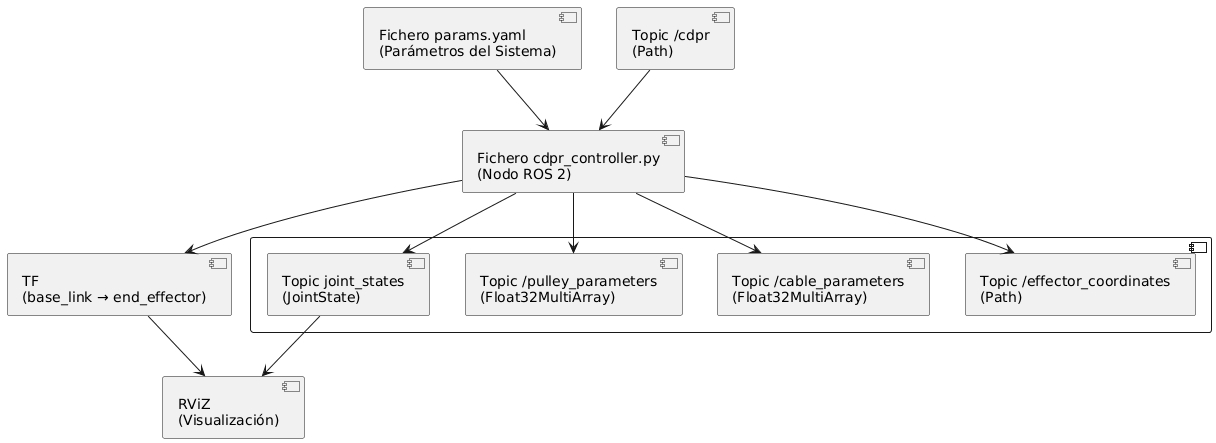
\includegraphics[width=\textwidth]{figs/general_system_architecture.png}
    \end{center}
    \caption{Arquitectura general del sistema en ROS 2}
\end{figure}\

Como se puede observar, se tiene una única posición o un conjunto de posiciones objetivo definidas por el usuario, las cuales se envían al nodo principal del sistema implementado, encargado de aplicar el modelo cinemático del robot para calcular las longitudes y los ángulos respecto a la vertical de cada cable, al igual que los ángulos de rotación y la cantidad de cable elongada o recogida por cada polea.

\newpage

Una vez calculados estos parámetros, toda esta información se publica mediante topics, lo que permite a otros componentes del sistema poder utilizar esta información, mientras se visualiza en RViZ el estado del sistema en cada momento utilizando el modelo URDF definido, lo que permite observar el comportamiento de todos los elementos que componen el sistema durante la ejecución de una trayectoria.

\section{Componentes software}
\label{sec:segundaseccion}

El desarrollo software es lo que compone en su gran mayoría al núcleo de este TFG, el cual se ha llevado a cabo en Python, ya que es un lenguaje de programación de alto nivel que se integra perfectamente con ROS 2 y que se caracteriza principalmente por su flexibilidad y legibilidad en código, siendo éstos los factores principales que he tenido en cuenta a la hora de elegir este lenguaje de programación antes que otros, como han sido MATLAB o C++.

\vspace{0.25cm}

El sistema software está compuesto principalmente por los siguientes elementos, los cuales trabajan de forma coordinada con el objetivo de ofrecer una simulación bastante coherente:

\begin{itemize}
\item Un nodo ROS 2 encargado de gestionar la ejecución del sistema, el cual recibe como entrada la posición o la trayectoria por la que se quiere desplazar el efector final.
\item Un fichero de configuración que permite ajustar los parámetros del sistema y personalizar la visualización.
\item Un modelo descriptivo del robot en URDF utilizado para su representación en RViZ.
\end{itemize}

\section{Sistema hardware}
\label{sec:segundaseccion}

El sistema hardware comprende una estructura rígida, en este caso una pizarra móvil con ruedas, encargada de sujetar los dos servomotores situados en las esquinas superiores de la misma que actúan como poleas, que a su vez se encargan de accionar los cables que definen la posición del efector final en cada momento, el cual se desplaza libremente dentro de la región bidimensional definida por el área de la pizarra.

\newpage

Aunque la construcción física del sistema real no esté completa a día de hoy, todo su diseño se ha definido en consonancia con todo el software desarrollado, ya que la posición de cada una de las poleas, el espacio de trabajo equivalente a las dimensiones de la pizarra y el tamaño del efector final se han tenido en cuenta desde las primeras fases de este TFG.

\section{Flujo general de funcionamiento}
\label{sec:segundaseccion}

En primer lugar, se recibe como entrada del sistema una o varias posiciones objetivo por las que el efector final debe pasar, a partir de las cuales el sistema aplica el modelo cinemático, obteniendo así todos los parámetros necesarios que permiten al sistema accionar los cables con el objetivo de que el efector final pase por todas las posiciones recibidas.

\vspace{0.25cm}

Con todos estos parámetros ya calculados, el sistema se va actualizando en cada momento mientras va publicando información relevante, como la posición del efector final, el valor de la longitud de cada cable y el ángulo girado por cada polea en tiempo real. Todo este flujo de trabajo se repite contínuamente hasta que el efector final llegue a la última posición que haya recibido por su entrada.

\vspace{0.25cm}

Es por ello que, para representar el comportamiento del sistema durante su ejecución, se adjunta a continuación un diagrama de flujo que describe todo este proceso.

\begin{figure} [h!]
    \begin{center}
        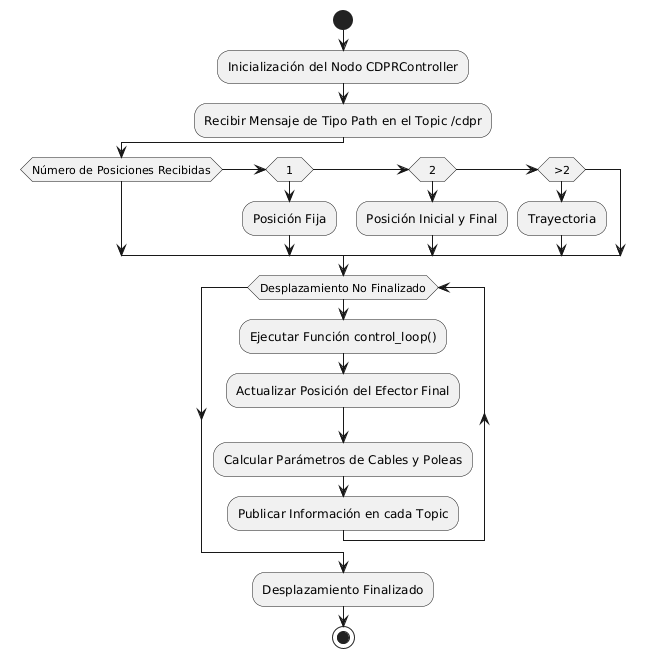
\includegraphics[width=\textwidth]{figs/general_system_workflow.png}
    \end{center}
    \caption{Flujo general de funcionamiento del sistema}
\end{figure}\

\newpage

Como se puede observar, el nodo recibe una única posición o una trayectoria objetivo, a partir de la cual se aplica el modelo cinemático para calcular la longitud de cada cable y los ángulos de rotación de cada polea.

\vspace{0.25cm}

Una vez hecho esto, el sistema publica los resultados obtenidos en topics, permitiendo así conocer el estado del sistema en tiempo real, al igual que en RViZ, donde se puede observar el movimiento del efector final y de las poleas en cada momento de la ejecución del sistema.

\section{Relación entre módulos}
\label{sec:segundaseccion}

Aunque gran parte de toda la funcionalidad del sistema se implemente en un único nodo, se pueden identificar claramente las relaciones entre todos los módulos que lo componen, como son las posiciones recibidas por su entrada, el cálculo cinemático y su visualización, lo que permite analizar y depurar el comportamiento del sistema de una forma mucho más estructurada, y que además, esta organización se puede seguir teniendo en cuenta en caso de que se quieran hacer ampliaciones en un futuro, como podría ser la adición de otro tipo de sensores en adición a los servomotores que ya se tienen, el paso de tener un sistema de control en lazo abierto a cerrado, o la separación del código en múltiples nodos ROS 2 en lugar de uno solo.
